\section{Grundlagen\label{francis:section:grundlagen}}
\rhead{Grundlagen}
Um ein besseres Verständnis für den Algorithmus zu bekommen, wollen wir uns zuerst einige wichtige Resultate aus der linearen Algebra in Erinnerung rufen.

\subsection{Ähnlichkeitstransformation\label{francis:section:grundlagen:aehnlichkeitstransform}}
\index{Ähnlichkeitstransformation}%
\index{similarity transformation}%
Wird eine Matrix von rechts mit einer Matrix $C$ multipliziert und von links mit der Inversen $C^{-1}$, handelt es sich um eine Ähnlichkeitstransformation. Die Transformation ist auch bekannt als Basiswechsel bzw. Similarity Transformation
\begin{equation}
	\hat{A}=C^{-1}AC.
\end{equation}
Oft wird die Transformation auch in der Form $C\hat{A}=AC$ dargestellt, welche sich durch einfaches Umformen erreichen lässt.
Es handelt sich bei einer solchen Transformation lediglich um einen Wechsel des Koordinatensystems.
Daher sind einige Eigenschaften einer Matrix gegenüber einer solchen Transformation invariant.
Zueinander ähnliche Matrizen haben:
\begin{enumerate}
	\item die gleiche Determinante
\index{Determinante}%
	\item die gleiche Spur
\index{Spur}%
	\item den gleichen Rang
\index{Rang}%
	\item das gleiche Minimalpolynom
\index{Minimalpolynom}%
	\item die gleiche jordanische Normalform
\index{Normalform, jordansche}%
\index{jordansche Normalform}%
	\item \textbf{die gleichen Eigenwerte (aber nicht notwendigerweise die gleichen Eigenvektoren)}
\end{enumerate}

Eigenwerte und Eigenvektoren können gefunden werden, indem man eine Matrix durch Ähnlichkeitstransformation auf Diagonalform bringt.
\index{Diagonalform}%
Der Francis-Algorithmus tut dies Schrittweise unter Verwendung sehr spezieller Matrizen $C$.

\subsection{Spezielle Matrizen\label{francis:section:grundlagen:spezielle_matrizen}}
Im Folgenden werden wir immer wieder über einige spezielle Matrixformen sprechen.
Reden wir von einer Matrix in der oberen Hessenberg-Form, meinen wir eine Matrix der Form:
\index{Hessenberg-Form, obere}%
\index{obere Hessenberg-Form}%
\begin{equation}
	\begin{bmatrix}
	* & * & * & * & * \\
	* & * & * & * & * \\
	& * & * & * & * \\
	&   & * & * & * \\
	&   &   & * & *
	\end{bmatrix},
\end{equation}
wobei die Sterne bedeuten, dass an dieser Stelle ein Wert in der Matrix steht, welcher nicht Null ist.
Die Form entspricht also fast einer oberen Dreiecksmatrix, zusätzlich sind aber alle Elemente unmittelbar unter der Diagonalen von Null verschieden.
Mit dem weiter unten im Abschnitt \ref{francis:section:vorbereitung} vorgestellten Verfahren kann eine allgemeine Matrix in obere Hessenberg-Form gebracht werden. Wendet man das gleiche Verfahren aber auf eine symmetrische Matrix an, entsteht eine Spezialform, eine Tridiagonalmatrix:
\index{Tridiagonalmatrix}
\begin{equation}
	\begin{bmatrix}
	* & * &   &   &   \\
	* & * & *  &   &   \\
	& * & * & * &  \\
	&   & * & * & * \\
	&   &   & * & *
	\end{bmatrix}.
\end{equation}

\subsection{Eigenwerte\label{francis:section:grundlagen:eigenwerte}}
Bei den Eigenvektoren einer Matrix handelt es sich um Vektoren, welche bei einer Multiplikation mit der Matrix die Richtung nicht ändern, sondern lediglich gestreckt werden.

\begin{satz}
	Ein Vektor $v$ $\subset \mathbb{C}^n$ ist ein Eigenvektor von A, wenn v $\neq$ und $Av$ ein Vielfaches von $v$ ist. Der Skalar $\lambda$ ist der zum Eigenvektor $v$ gehörende Eigenwert von $A$
\end{satz}

Es gilt also:
\begin{equation}
	Av=\lambda v.
\end{equation}
Gesucht sind die Nullstellen des charakteristischen Polynoms
\index{charakteristisches Polynom}%
\begin{equation}
	\chi_A(\lambda)=\det(A-\lambda I) = 0.
\end{equation}
 Da ein Polynom vom Grad $n$ höchstens $n$ Nullstellen hat, gibt es auch höchstens $n$ Eigenwerte.

\begin{beispiel}
Die Eigenwerte einer kleinen Matrix
	\begin{equation}
	A =
	\begin{bmatrix}
	1 & 3 & 2 \\
	0 & 2 & 1 \\
	0 & 0 & 3
	\end{bmatrix}
	\end{equation}
können wie folgt berechnet werden.
	
	\begin{equation}
	\det(A-\lambda I)= \det
	\begin{pmatrix}
	\begin{bmatrix}
	1-\lambda & 3 & 2 \\
	0 & 2-\lambda & 1 \\
	0 & 0 & 3-\lambda
	\end{bmatrix}
	\end{pmatrix}
	= 0
	\end{equation}	
daraus folgt:
	
	\begin{equation} 
	(1-\lambda)(2-\lambda)(3-\lambda)=0
	\end{equation}
und die Eigenwerte sind mit $\lambda_{1}=1$, $\lambda_{2}=2$ und $\lambda_{3}=3$ gefunden.
\end{beispiel}

Wie im Beispiel ersichtlich, sind die Eigenwerte einer Matrix in Dreiecks- oder Diagonalform durch die Diagonalelemente gegeben.
Da bei Bestimmung der Determinante (bei 3. Ordnung z. B. mit der Regel von Sarrus) alles andere verschwindet.
\index{Sarrus, Regel von}%
\index{Regel von Sarrus}%

\subsection{Givens-Rotationen\label{francis:section:grundlagen:givens}}
\index{Givens-Rotation}%
Rotationsmatrizen sind attraktiv, da sie einfach konstruiert werden können und mit ihnen durch eine geeignete Wahl des Rotationswinkels an einer gewünschten Stelle in einem Vektor eine Null erzeugt werden kann.
Dazu wird eine Rotations- bzw. Drehmatrix verwendet.
Sie hat in zwei Dimensionen die folgende Form:
\begin{equation}
	R=\begin{bmatrix}
	\cos\phi & -\sin\phi \\
	\sin\phi & \cos\phi
	\end{bmatrix}.
\end{equation}
Zur Drehung eines Punktes $P=(x,y)$ um den Winkel $\phi$ kann man einfach den dazugehörigen Ortsvektor mit der Rotationsmatrix multiplizieren und erhält so den Ortsvektor des gedrehten Punktes.
Es handelt sich dabei um eine Givens-Rotationsmatrix, wenn $R^{-1}(\phi)=R_{T}(\phi)=R(-\phi)$.
Durch Erweiterung der Rotationsmatrix können Drehungen natürlich auch in einem höherdimensionalem Raum verwendet werden.

\begin{beispiel}
Gegeben sei die Multiplikation einer Rotationsmatrix mit einem beliebigen Vektor:
	\begin{equation}
	\begin{bmatrix}
	1 & 0 & 0 & 0 & 0 & 0 \\
	0 & \cos\phi & 0 & 0 & -\sin\phi & 0 \\
	0 & 0 & 1 & 0 & 0 & 0 \\
	0 & 0 & 0 & 1 & 0 & 0 \\
	0 & \sin\phi & 0 & 0 & \cos\phi & 0 \\
	0 & 0 & 0 & 0 & 0 & 1 \\
	\end{bmatrix}
	\begin{bmatrix}
	x_{1}\\
	x_{2}\\
	x_{3}\\
	x_{4}\\
	x_{5}\\
	x_{6}\\
	\end{bmatrix}
	=
	\begin{bmatrix}
	x_{1}\\
	x_{2}\cos\phi-x_{5}\sin\phi\\
	x_{3}\\
	x_{4}\\
	x_{2}\sin\phi+x_{5}\cos\phi\\
	x_{6}\\
	\end{bmatrix}.
	\end{equation}	
Wie dabei zu sehen ist, werden dabei nur die 2. und 5. Spalte des Vektors verändert.
Eine Anwendung einer solchen Rotationsmatrix entspricht also einer Rotation in jener Ebene im 6-dimensionalen Raum, welche von Achse 2 und 5 aufgespannt wird.
Durch eine geeignete Wahl des Rotationswinkels und ein systematisches Anwenden diverser Rotationsmatrizen kann man so einen Eintrag nach dem Andern auf Null setzen und beispielsweise eine QR-Zerlegung durchführen. \cite{francis:QR_Zerlegung} 
Weiteres dazu ist in den Kapiteln \ref{buch:section:qr} und \ref{chapter:qr} zu finden.
\end{beispiel}

\subsection{Householder-Transformation\label{francis:section:grundlagen:householder}}
\index{Householder-Transformation}%
Reflektoren (siehe Abschnitt \ref{buch:subsection:spiegelungn}) sind attraktiv, da sie einfach konstruiert werden können und mit ihnen alle Elemente eines Vektors bis auf ein Element auf Null gesetzt werden können.
So kann jede beliebige Matrix relativ einfach in Hessenberg-Form gebracht werden.
Ein beliebiger Vektor $x$ und ein spezieller Vektor $y$ sind gegeben:
\begin{equation}
	x=
	\begin{bmatrix}
	x_{1}\\
	x_{2}\\
	\vdots\\
	x_{n}\\
	\end{bmatrix}
	,\qquad y=
	\begin{bmatrix}
	y_{1}\\
	0\\
	\vdots\\
	0\\
	\end{bmatrix}\qquad \text{mit } y_{1}\pm \norm{x}	
\end{equation}
Da diese beiden Vektoren dieselbe Länge haben, wissen wir, dass ein Reflektor $H$ existiert, sodass $Hx=y$.
Mit dem Reflektor
\begin{equation}
	H=I-2vv^{T}, \qquad \text{mit } v=(x-y)/\norm{x-y}
\end{equation}
können also alle Elemente eines Vektors bis auf ein Element auf null gesetzt werden.
Das Ganze ist in Abbildung \ref{francis:abb:householder_transform} in zwei Dimensionen dargestellt.
\begin{figure}[h]
	\begin{center}
		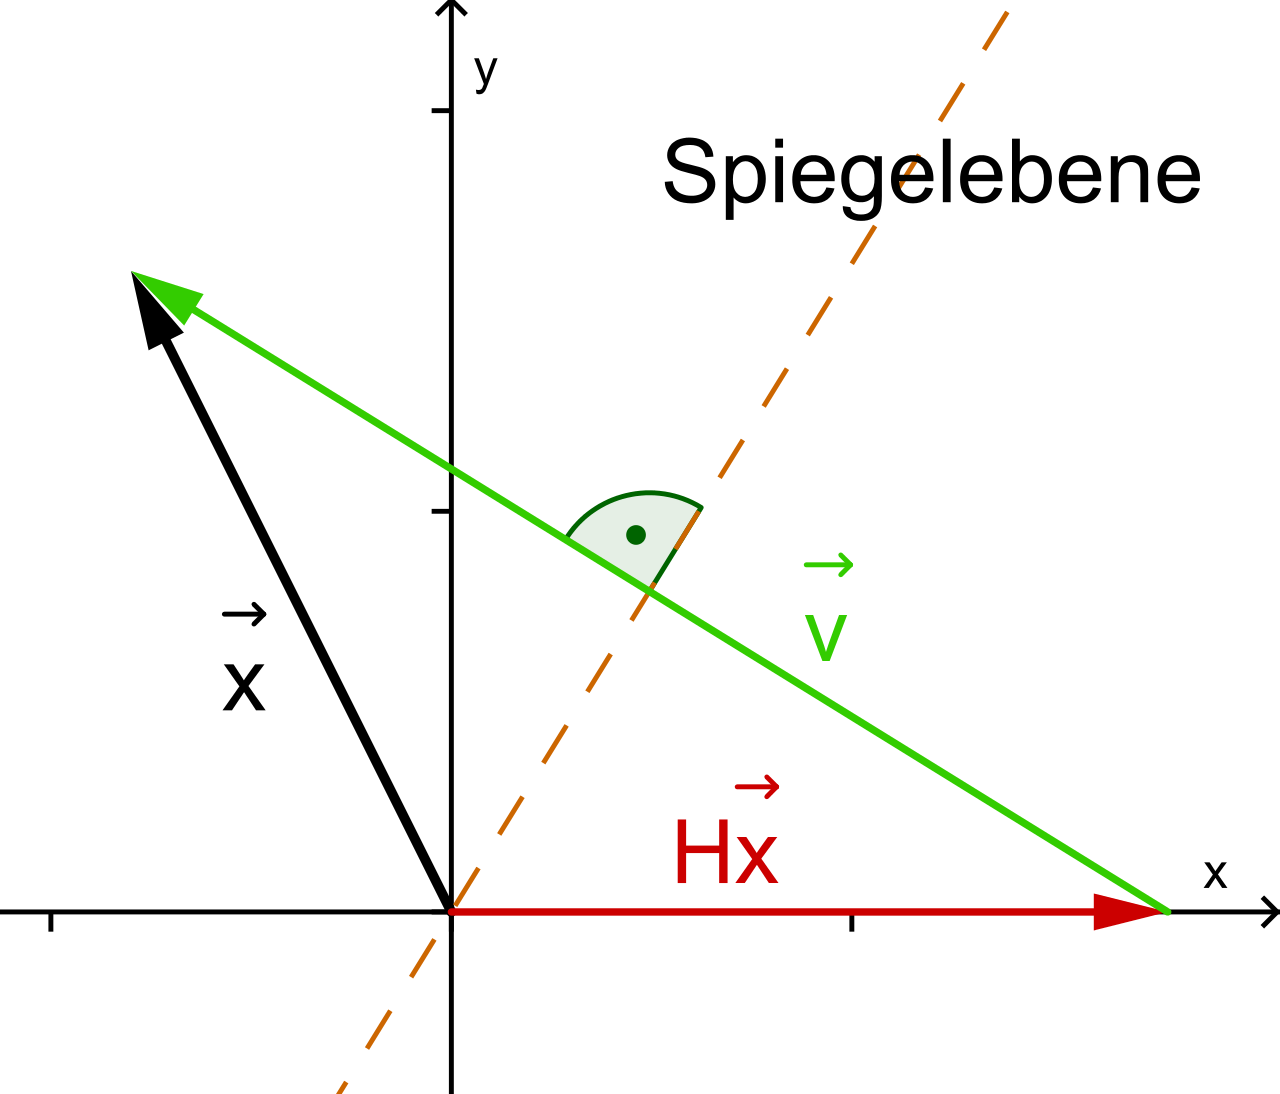
\includegraphics[scale=0.1]{papers/francis/images/Householdertransformation.png}
		\caption{Illustration der Householder-Transformation in zwei Dimensionen, Abbildung von \cite{francis:householder}}
		\label{francis:abb:householder_transform}
	\end{center}
\end{figure}
